

\section{Preguntas de desarrollo}

\begin{enumerate}
%-------------------------------------------------------------------------------------
	\item \textbf{ Investigue y Explique los tipos de fibras de dispersión desplazada que existen, muestre comparativos (sus diagramas de dispersión v/s $\lambda$ y sus perfiles de índice de refracción núcleo-manto),ventajas y desventajas de cada una, la normativa UIT-T G.6XX asociada a cada una y cuál tipo fibra de dispersión desplazada recomendaría usted a Codelco para el enlace de fibra óptica con transporte DWDM y posible uso de amplificador proyectado. Justifique}\\\\
	La dispersión desplazada es una técnica en fibras ópticas monomodo diseñada para controlar y minimizar la dispersión cromática en una longitud de onda específica, usualmente en el rango de 1550 nm, que es ideal para transmisiones de telecomunicaciones. Este tipo de fibra optimiza el rendimiento en esa longitud de onda, lo que permite una transmisión de señal más eficiente y de mayor alcance, especialmente útil en redes de larga distancia. Entre sus ventajas está la reducción de la distorsión en la señal a esa longitud de onda, lo que facilita el envío de datos de alta velocidad sin necesidad de amplificación frecuente. Sin  embargo, una desventaja importante es que, debido a su baja dispersión en la banda de 1550 nm, estas fibras pueden sufrir de efectos no lineales, como \textit{four-wave mixing}, en sistemas que usan múltiples longitudes de onda (DWDM), lo cual puede causar interferencia entre canales y limitar su uso en aplicaciones de alta densidad.
	\begin{figure}
		\centering
		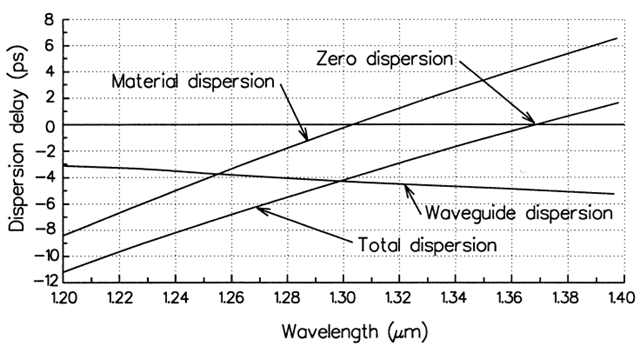
\includegraphics[width=0.7\linewidth]{img/Figure_1_0}
		\caption{Fibra óptica monomodo de dispersión desplazada}
		\label{fig:1}
	\end{figure}
	\begin{itemize}
		\item \textbf{Normativa UIT-T G.653:} Establece los estándares para la fibra óptica monomodo de dispersión desplazada convencional (DSF). Esta fibra está diseñada para que la dispersión cromática sea prácticamente nula en la banda de los 1550 nm, lo cual es óptimo para la transmisión en telecomunicaciones, especialmente en aplicaciones de larga distancia y alta velocidad. Gracias a esta característica, la fibra G.653 ofrece una transmisión eficiente y con baja distorsión en esa banda. Sin embargo, su dispersión tan baja la hace más susceptible a efectos no lineales, como la mezcla de cuatro ondas (Four-Wave Mixing), lo que puede causar interferencia en sistemas de multiplexación por división de longitud de onda (WDM). Por esta razón, aunque es muy útil en ciertos contextos de telecomunicaciones, su aplicación puede ser limitada en sistemas de alta densidad de canales.
		
		\item \textbf{Normativa UIT-T G.655:} Esta normativa se centra en las fibras de dispersión desplazada no nula (NZ-DSF). Estas fibras están diseñadas para aplicaciones de transmisión a larga distancia en sistemas DWDM, ya que tienen una dispersión cromática no nula que evita efectos no lineales, como la mezcla de cuatro ondas (FWM), que es problemática en fibras con dispersión nula. Existen variantes con dispersión cromática positiva o negativa, lo que permite adaptar la fibra a diferentes requerimientos de red. Aunque su producción es más costosa debido a la complejidad del diseño, la UIT-T G.655 es una excelente opción para enlaces de alta densidad en DWDM, como el proyectado para Codelco en el proyecto Rajo Inca.
		
		\item \textbf{Normativa UIT-T G.656:} Esta normativa cubre fibras ópticas diseñadas para proporcionar una dispersión controlada en un rango de longitudes de onda extendido, usualmente entre 1460 nm y 1625 nm. Este tipo de fibra es particularmente útil para aplicaciones de alta capacidad en redes metropolitanas y de larga distancia, ya que su diseño permite reducir la necesidad de compensación de dispersión, mejorando la eficiencia de los sistemas DWDM. Su uso es preferido en redes donde se necesita flexibilidad en la longitud de onda operativa, especialmente cuando se requiere optimizar el rendimiento en un amplio espectro de frecuencias.
	\end{itemize}
	
	\begin{figure}
		\centering
		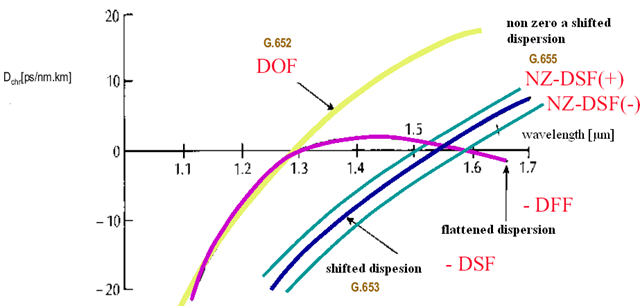
\includegraphics[width=0.7\linewidth]{img/Figure_1_1}
		\caption{Fibra óptica monomodo de dispersión desplazada para diferentes aplicaciones}
		\label{fig:2}
	\end{figure}
	
	\begin{table}[H]
		\centering
		\begin{tabular}{|c|p{6cm}|p{6cm}|}
		\hline
		\textbf{Normativa} & \textbf{Ventajas} & \textbf{Desventajas} \\
		\hline
		UIT-T G.653 & 
		Dispersión prácticamente nula a 1550 nm, ideal para transmisión en largas distancias y alta velocidad. & 
		Susceptibilidad a efectos no lineales como la mezcla de cuatro ondas, limitando su uso en sistemas WDM de alta densidad. \\
		\hline
		UIT-T G.655 & 
		Dispersión no nula pero controlada, reduciendo interferencias en sistemas DWDM. & 
		Costo de producción elevado debido a su diseño especializado. \\
		\hline
		UIT-T G.656 & 
		Flexibilidad para ajustarse a diversas configuraciones de red con dispersión positiva o negativa según necesidad. & 
		Diseño especializado implica un costo más alto, aunque mejora el rendimiento en sistemas complejos. \\
		\hline
		\end{tabular}
		\caption{Ventajas y desventajas de las normativas UIT-T G.653, G.655 y G.656}
	\end{table}
	
	Para el enlace de fibra óptica DWDM que necesita Codelco en el proyecto Rajo Inca, la fibra recomendada es la fibra de dispersión desplazada no cero (NZ-DSF), regulada bajo la normativa UIT-T G.655. Esta opción es ideal porque su dispersión controlada en la banda de 1550 nm minimiza efectos no lineales, como \textit{Four-Wave Mixing }, evitando interferencias en sistemas DWDM de alta densidad.
	
%-------------------------------------------------------------------------------------
	\item \textbf{Describa la forma de operación de los siguientes equipos ópticos más comúnmente utilizados: Fuente LED, Fuente VCSEL, Fuente LASER, Fotodiodo PIN y
	Fotodiodo APD. Adicionalmente, para las Fuentes óptica recomiende la longitud de onda de la fuente y tipo de fibra para ser utilizada, y para los Fotodiodos presente una tabla comparativa.}\\\\
	Las fuentes ópticas son dispositivos que generan luz para la transmisión de datos a través de fibras ópticas. Funcionan convirtiendo señales eléctricas en señales ópticas, que se propagan a lo largo de la fibra para transportar información en forma de pulsos de luz. Algunas de estas son:
	\begin{itemize}
		\item \textbf{Fuente LED:} Las fuentes de luz LED (Light Emitting Diode) son dispositivos que emiten luz mediante la recombinación de electrones y huecos en una unión p-n, generando una luz incoherente con un espectro amplio. Este tipo de fuente es común en aplicaciones de corto alcance, donde la velocidad de transmisión y la distancia no son muy altas, como en redes de área local y conexiones de bajo costo. La luz generada por los LEDs tiene una divergencia mayor en comparación con otras fuentes, lo que la hace adecuada para fibras multimodo, siendo una opción accesible y duradera.
		\item \textbf{Fuente laser:} Emite luz coherente y monocromática a través de la emisión estimulada, produciendo un haz de luz de alta potencia y estrecho espectro. Gracias a estas características, los láseres son ideales para aplicaciones de telecomunicaciones que requieren alta velocidad y transmisiones de larga distancia. Las longitudes de onda recomendadas para fuentes láser en telecomunicaciones son 1310 nm y 1550 nm, las cuales se utilizan en combinación con fibras monomodo para minimizar la dispersión y maximizar el alcance y la calidad de la señal.
		\item \textbf{Fuente VCSEL:} Los VCSEL (Vertical-Cavity Surface-Emitting Laser) son una variante de los láseres que emiten luz perpendicular a la superficie del chip, lo que permite una mayor eficiencia y control de la emisión. Estos dispositivos son comunes en aplicaciones de corto alcance, como redes de área local y conexiones de alta velocidad, donde se requiere una alta densidad de canales y una fácil integración con sistemas ópticos. Los VCSELs son una opción económica y versátil para aplicaciones de corto alcance, con longitudes de onda típicas de 850 nm y 1300 nm.
	\end{itemize}
	\begin{figure}
		\centering
		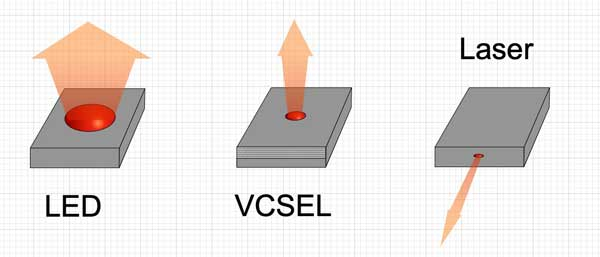
\includegraphics[width=0.7\linewidth]{img/Figure_2_0}
		\caption{Comparación de fuentes ópticas LED, VCSEL y láser}
		\label{fig:3}
	\end{figure}
	Los detectores ópticos son dispositivos que convierten la luz en señales eléctricas, permitiendo la recepción y decodificación de datos transmitidos a través de fibras ópticas. Funcionan absorbiendo los fotones de la señal óptica y generando una corriente eléctrica proporcional a la intensidad de la luz recibida. Algunos ejemplos de estos son:
	\begin{itemize}
		\item \textbf{Fotodiodo PIN:} Los fotodiodos PIN son detectores de alta velocidad y baja capacidad que convierten la luz en corriente eléctrica mediante la absorción de fotones en una región de alta dopaje. Este detector es comúnmente usado en aplicaciones de baja a media distancia y en sistemas donde la sensibilidad no es crítica, como en redes de datos LAN.
		\item \textbf{Fotodiodo APD:} Los fotodiodos APD son detectores de alta sensibilidad que utilizan el efecto de avalancha para amplificar la señal óptica. Estos dispositivos son ideales para aplicaciones de alta velocidad y baja intensidad, donde se requiere una alta sensibilidad y una respuesta rápida. 
	\end{itemize}
\begin{figure}
	\centering
	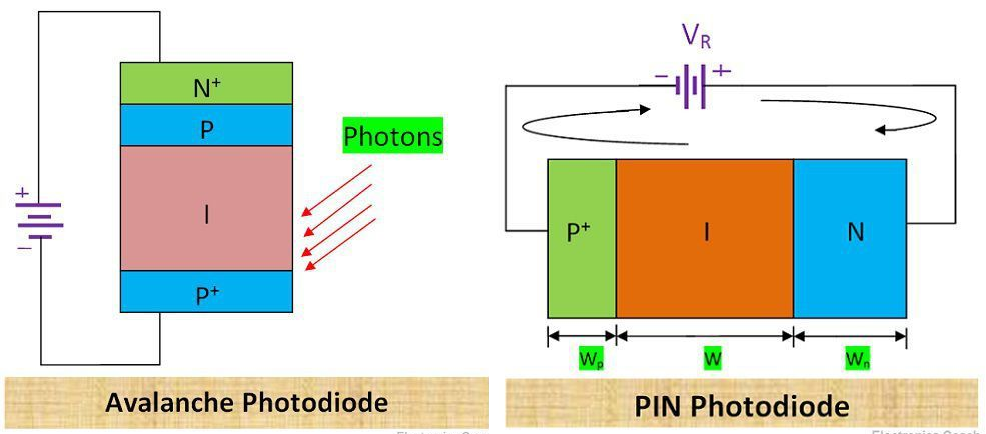
\includegraphics[width=0.7\linewidth]{img/Figure_2_1}
	\caption{Comparación de fotodiodos PIN y APD}
	\label{fig:4}
\end{figure}
	Sera util el utilizar una fuente láser de 1550 nm y un fotodiodo APD. La fuente láser es ideal para largas distancias y sistemas DWDM, ya que proporciona luz coherente y de baja dispersión. El fotodiodo APD, por su alta sensibilidad, garantiza una recepción confiable en un enlace de gran distancia.
%-------------------------------------------------------------------------------------
	\item \textbf{Los Ingenieros de Codelco le presentan el siguiente sistema óptico como bosquejo de diseño para comunicar el Rajo Inca con el Datacenter cercano a Copiapó (140 Km) con fibra monomodo y uso de $\lambda$ transporte en banda C con frecuencia central nominal a 193.2 Thz revisar norma ITU-T G.694.1}
	\begin{figure}
		\centering
		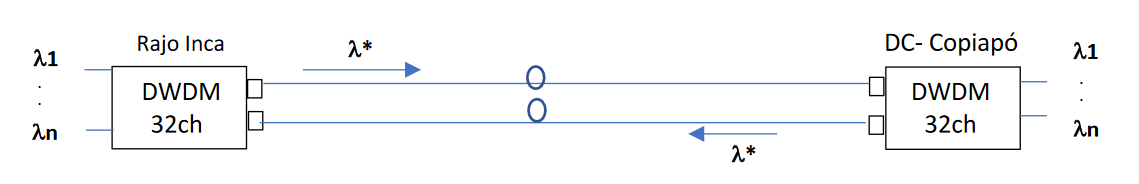
\includegraphics[width=0.7\linewidth]{img/Figure_3_0}
		\caption{Sistema óptico para enlace Rajo Inca - Datacenter}
		\label{fig:5}
	\end{figure}
	\begin{itemize}
		\item Le solicitan calcular la Potencia óptica de salida para el diseño propuesto para una Potencia de entrada de 2,5dBm. Comente si la potencia de salida está dentro de los rangos permitidos del transponder\\\\
		Se busca obtener la potencia óptica de salida del sistema óptico propuesto, considerando una potencia de entrada de 2,5 dBm. Para ello,se deberan tener en consideraicon todas las perdidas presentes, es decir:
		\begin{itemize}
			\item Las perdidas por la fibra vendran dadas por:
			\begin{align}
				\text{Perdidas fibra} = 0.2 [dB/Km] \times 140[Km] = 28 \text{dB}
			\end{align}
			\item Las perdidas por los conectores vendran dadas por:
			\begin{align}
				\text{Perdidas conectores} = 0.5 [dB] \times 2 = 1 \text{dB}
			\end{align}
			\item Perdidas por lo empalmes que vienen dado por un total de $\frac{140[km]}{20[Km]}$-1 = 6
			\begin{align}
				\text{Perdidas empalmes} = 0.03 [dB] \times 6  = 0.18 \text{dB}
			\end{align}
		\end{itemize}
		De esta manera se tienen que las perdidas totales seran:
		\begin{align}
			\text{Perdidas totales} = 28 + 1 + 0.18 = 29.18 \text{dB}
		\end{align}
		Considerando que la potencia de entrada es de 2.5 dBm, la potencia de salida sera:
		\begin{align}
			\text{Potencia de salida} = 2.5 - 29.18 = -26.68 \text{dBm}
		\end{align}
		La potencia de salida obtenida es de -26.68 dBm, lo que se encuentra dentro del rango permitido para un transponder (-30 dBm a -10 dBm) y garantiza una transmisión eficiente y confiable en el enlace de 140 km.
		\item Analice un diagrama teórico alternativo para cambiar de Datacenter a uno de 190Km del Rajo Inca, la cuál se considere colocar un amplificador de línea EDFA (FWA-1550L-20) de 20dBm de Ganancia\\\\
		Se busca el analizar un diagrama teórico alternativo para un enlace de 190 km desde el Rajo Inca a un Datacenter, considerando la instalación de un amplificador de línea EDFA (Erbium-Doped Fiber Amplifier) con una ganancia de 20 dBm. Para esto deberemos considerar que la potencia de salida del primer tramo debe estar 4dB por encima de la sensibilidad del transponder, por lo tanto:
		\begin{align}
			P_{requisito} = S_{e} + 4dB
		\end{align}
		Dado que la sensibilidad del transponder es $S_{e}= -30dB$ tendremos que:
		\begin{align}
			P_{requisito} = -30dB + 4dB = -26dB
		\end{align}
		Por lo tanto se calculara la distancia maxima para que podamos tener una potencia de salida de -26dBm y ubicar el amplificador. Se tiene que:
		\begin{align}
			P_{salida} = 2.5dBm - P_{perdidas}
		\end{align}
		Dado que nos interesa cuanado la potencia de salida es de -26dBm se tiene que la atenuacion total que podemos tener sera de 28.5dB , ademas deberemos considerar los efectos del empalme como la de 1 conexion (), por tanto se formula la siguiente ecuacion:
		\begin{align}
			28.5 &= P_{conector} + P_{empalme} + P_{fibra}\\
			28.5 &= 0.5 + 0.03(n-1) + 0.2 \cdot 20n\\
			n&= 6.95
		\end{align}
		Con lo que el amplificador se debera instalar a una distancia de 139 km. Luego para el segundo tramo tenemos lo siguiente:
		\begin{align}
			P_{equisito} = S_{e} + 2dB = -30dB + 2dB = -28dB
		\end{align}
		Luego dado que el amplificador EDFA tiene una ganancia de 20dBM y considerando que esta recibiendo una señal de -26dBm, se tiene que la potencia de salida sera de -6dBm, luego tendremos que la atenuacion para el segundo tramo debera ser de almenos:
		\begin{align}
			P_{\text{Salida amplificador}} - P_{\text{requisito segundo tramo}}= -6[dbm] -(-28[dbm]) = 22[db]
		\end{align}
		De esta manera podemos tener almenos 22dB de perdidas, por lo que la distancia maxima para el segundo tramo sera de:
		\begin{align}
			22 &= P_{conector} + P_{empalme} + P_{fibra}\\
			22 &= 0.5 + 0.03(n-1) + 0.2 \cdot 20n\\
			n&=5.34
		\end{align}
		Esto entrega una distancia maxima de 106.8 km, por lo que el segundo tramo debera ser de 106.8 km. Pero se observa que cumple con la distancia maxima de 190 km por lo que el utilizar un amplificador a una distancia de 139 km es una buena opcion y mas que suficiente para el enlace de 190 km.
	\end{itemize}
	%-------------------------------------------------------------------------------------
	\item \textbf{Los ingenieros le solicitan que realice el cálculo de dispersiones y tiempos de subida que les permita concluir que la fibra óptica y transponder escogidos son los adecuado para la transmisión de un BW de 10Gbps a 140Km}
		\begin{itemize}
			\item Obtenga el Cálculo de Dispersión Total\\\\
			Dado que se busca calcular la dispersión total de la fibra óptica para determinar si es adecuada para la transmisión de 10 Gbps a 140 km, se deben considerar los siguientes factores:
			\begin{align}
				T_{crom} &= (Coef_{material} + Coef_{guia}) \cdot W_{espectral} \cdot l\\
						&= (6[ns/(nm \cdot km)] - 5.99[ns/(nm \cdot km)]) \cdot 0.01[nm] \cdot 140[km]\\ 
						&= 0.014ns\\
						&= 14 ps
			\end{align}
			Luego para la $T_{PMD}$ se tendra que:
			\begin{align}
				T_{PMD} &= 0.75 ps/\sqrt{km} \cdot \sqrt{140 [km]} \\
				&= 8.87412 ps
			\end{align}
			De esta manera tenemos finalmente que la dispersion total sera:
			\begin{align}
				T_{total} &= \sqrt{T^{2}_{cromática} + T^{2}_{PMD}}\\
				 &= \sqrt{14^{2} + 8.87412^{2}}\\
				 &= 16.5 ps
			\end{align}
			Con lo que se obtiene el valor de la dispersion total de la fibra óptica.
			\item Obtenga los Tiempos de Subida del Equipo, Compara con Tiempos de Subida de la FO y Concluya\\\\
			Dado que se busca obtener los tiempos de subida del equipo tenemos que viene dado por:
			\begin{align}
				T_{equipo} = T_{sys} - T_{gen} - T_{rx}
			\end{align}
			Luego se debe obtener $T_{sys}$ el cual correspondera a:
			\begin{align}
				T_{sys} = \frac{0.35}{BW} = \frac{0.35}{10 \times 10^{9}} = 35 ps
			\end{align}
			De esta manera se tendra que:
			\begin{align}
				T_{equipo} = 35[ps] - 2[ps] - 1[ps] = 32[ps]
			\end{align}
			Dado que $TE_{equipo}=32[ps]$ es mayor que $TF_{total}=16.5[ps]$, es posible el concluir que el tiempo de subida del equipo es suficiente para manejar la dispersión total de la fibra óptica en el enlace de 140 km a una tasa de 10 Gbps, asegurando una transmisión adecuada sin comprometer la integridad de la señal.
		\end{itemize}
		%-------------------------------------------------------------------------------------
		\item \textbf{Los ingenieros de Codelco saben que el uso de EDFA trae consigo desafortunadamente una emisión espontánea amplificada (ASE) y éste es un factor limitante del alcance y la capacidad de estos sistemas, traduciéndose en ruido óptico que distorsiona la señal del canal. Investigue y Explique de manera clara y sencilla los siguientes términos de medición usados en sistemas ópticos: OSNR, BER y Factor Q, y fundamente cuál es la relación que existe entre ellos.}\\\\
		
		Se busca describir y explicar los términos de medición utilizados en sistemas ópticos, como OSNR, BER y Factor Q, y su relación entre sí por lo tanto tenemos que:

		\begin{itemize}
			\item \textbf{OSNR (Optical Signal-to-Noise Ratio):} Es una medida de la relación entre la potencia de la señal óptica y la potencia del ruido en un sistema de comunicaciones ópticas. Se expresa en decibelios (dB) y se utiliza para evaluar la calidad de la señal y la relación señal-ruido en un enlace de fibra óptica. Un OSNR alto indica una señal fuerte y un ruido bajo, lo que se traduce en una mejor calidad de la señal y una menor probabilidad de errores en la transmisión. Por otro lado, un OSNR bajo puede causar interferencias y distorsiones en la señal, lo que afecta la integridad de los datos transmitidos.
			\begin{figure}
				\centering
				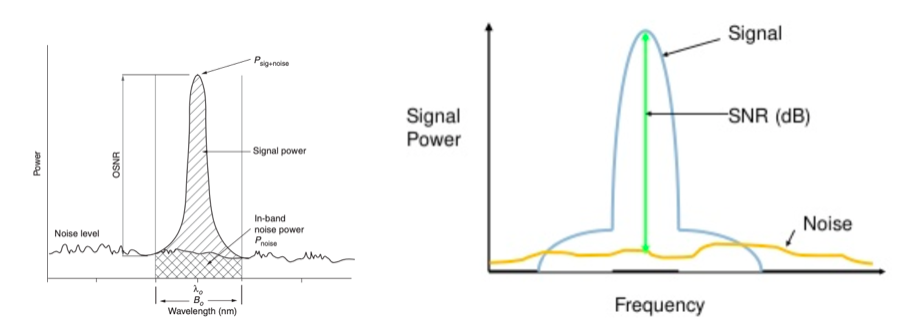
\includegraphics[width=0.7\linewidth]{img/Figure_5_0}
				\caption{Visualizacion de el OSNR en un sistema óptico}
				\label{fig:6}
			\end{figure}
			\item \textbf{BER (Bit Error Rate):} Es una medida de la tasa de errores en la transmisión de datos digitales a través de un canal de comunicaciones. Se expresa como la proporción de bits erróneos con respecto al total de bits transmitidos y se utiliza para evaluar la calidad y la fiabilidad de un sistema de comunicaciones. Un BER bajo indica una transmisión confiable y una alta integridad de los datos, mientras que un BER alto puede causar pérdida de información y errores en la recepción de los datos.
			\item \textbf{Factor Q:} Es una medida de la calidad de la señal en términos de la separación entre los niveles de señal "1" y "0". Se utiliza en sistemas digitales para indicar cuán bien se diferencian estos niveles de señal en la recepción. Un Factor Q alto implica que los niveles de "1" y "0" están bien definidos y separados, lo que reduce la probabilidad de errores en la interpretación de los bits recibidos.
			\begin{figure}
				\centering
				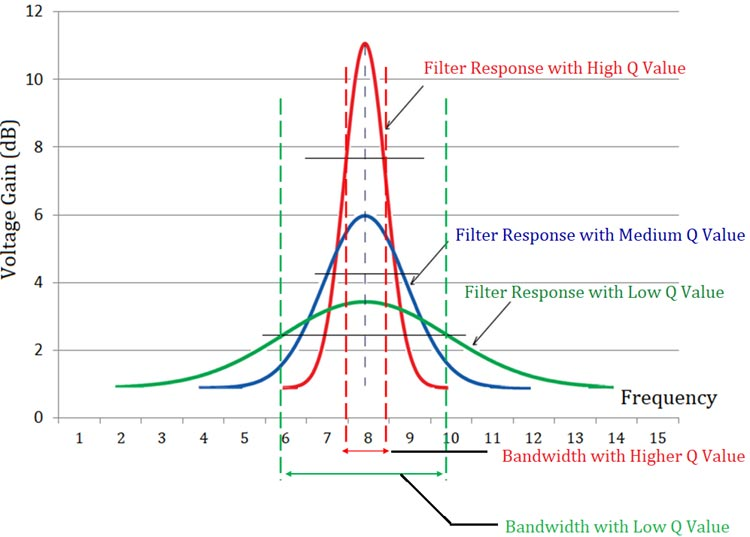
\includegraphics[width=0.5\linewidth]{img/Figure_5_1}
				\caption{Visualizacion de el Factor Q para diferentes calidades}
				\label{fig:7}
			\end{figure}
			\begin{table}[H]
				\centering
				\begin{tabular}{|c|p{5cm}|p{5cm}|}
				\hline
				\textbf{Parámetros} & \textbf{Relación} & \textbf{Efecto en la Calidad de Transmisión} \\
				\hline
				OSNR y BER & Un OSNR alto reduce el BER, ya que la señal es más fuerte que el ruido, facilitando una transmisión precisa. Un OSNR bajo aumenta el BER, pues el ruido afecta la claridad de la señal. & A mayor OSNR, menor BER, lo que mejora la calidad de la transmisión al reducir los errores de bits. \\
				\hline
				Factor Q y BER & Un Factor Q alto significa que los niveles de señal están bien definidos, resultando en un BER bajo. A medida que el Factor Q disminuye, el BER aumenta, indicando más errores en la recepción. & A mayor Factor Q, menor BER, lo que implica una transmisión más confiable y de alta calidad. \\
				\hline
				OSNR y Factor Q & Un OSNR alto mejora el Factor Q al reducir el ruido, facilitando la diferenciación de los niveles de señal. Un OSNR bajo disminuye el Factor Q, aumentando la dificultad para distinguir entre 1 y 0. & A mayor OSNR, mayor Factor Q, lo que aumenta la claridad de la señal y reduce la probabilidad de errores. \\
				\hline
				\end{tabular}
				\caption{Relación entre OSNR, BER y Factor Q en sistemas ópticos}
				\end{table}
		\end{itemize}
		Ademas se busca el obtener el valor de OSNR considerando solo 1 amplificador para el caso de los 190 km, se tiene que la expresion viene dada por:
		\begin{align}
			\text{OSNR} &= P_{\text{out}} - L - NF_{\text{eff}} - 10 \cdot \log_{10} \left( x + \frac{10^{G_{\text{BA}}/10}}{10^{L/10}} \right) - 10 \cdot \log_{10}(h \cdot \nu \cdot \nu_r) 
		\end{align}
		Esto segun la nortamtiva ITU-T G.696.1. Luego para su calculo se tiene que considerar lo siguiente:
		\begin{itemize}
			\item \textbf{\( N_{\text{eff}} \):} 5 dB
			\item \textbf{\( \nu \):} \( 193.2 \times 10^{12} \, \text{Hz} \)
			\item \textbf{h:} \( 6.63 \times 10^{-31} \, \text{mJ} \cdot \text{s} \)
			\item \textbf{\( \nu_{r} \):} 12.5 GHz
			\item \textbf{Potencia de entrada (\( P_{\text{out}} \)):} 2.5 dBm
			\item \textbf{Atenuación del tramo (L):} \( L = 0.2 \, \text{dB/km} \times 190 \, \text{km} = 38 \, \text{dB} \)
			\item \textbf{Ganancia del amplificador (\( G_{\text{BA}} \)):} 20 dB
			\item \textbf{Número de amplificadores (x):} 1
		\end{itemize}
		Con lo que reemplazando los valores tenemos que:
		\begin{align}
			\text{OSNR} &= 2.5 - 38 - 5 - 10 \cdot \log_{10} \left( 1 + \frac{10^{20/10}}{10^{38/10}} \right) \\
			&\quad - 10 \cdot \log_{10}(6.63 \times 10^{-31} \cdot 193.2 \times 10^{12} \cdot 12.5 \times 10^{9}) \\
			&= 2.5 - 38 - 5 - 0.06829 - (-87.955)\\
			&= 42.3867 \text{dB}
		\end{align}
		Dado el valor de OSNR obtenido, se puede concluir que el sistema de transmisión de 190 km con un amplificador EDFA cumple con los requisitos de calidad de señal y ruido.
		%-------------------------------------------------------------------------------------
		\item \textbf{Utilizando el Simulador OptiSystem diseñe el sistema óptico DWDM de 32ch (con sólo 2 canales habilitados) con un amplificador de línea EDFA (punto 3b) para presentar a cliente considerando los parámetros ópticos entregados}
		\begin{itemize}
			\item Captura de Pantalla de Diseño óptico global en OptiSystem, capturas de pantalla de los parámetros configurados por cada componente y use herramientas de visualización de potencias ópticas, pérdidas del sistema entre otros (con amplificador y sin amplificador).
			Compare y concluya lo obtenido entre los cálculos teóricos y las simulaciones.
		Se busca el implementar un sistema óptico DWDM de 32 canales con 2 canales habilitados. Para esto comenzaremos analizando el caso del sistema sim amplificador pero de 120 km, para esto se tiene que:
		\begin{figure}
			\centering
			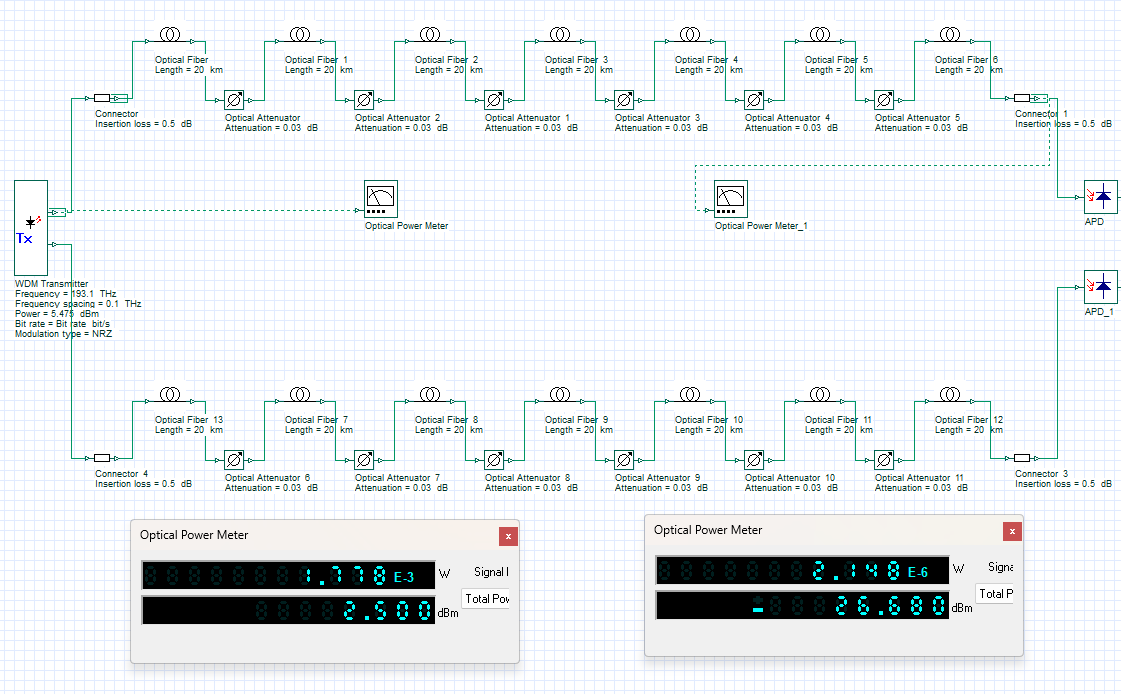
\includegraphics[width=0.9\linewidth]{img/Figure_6_0}
			\caption{Diseño óptico global en OptiSystem para la situacion sin amplificador una linea de 140Km}
			\label{fig:8}
		\end{figure}
		Se utiliza un \textit{Power meter} tanto en la entrada como en la salida y se visualizan en la figura (\ref{fig:8}) respectivamente, se obtiene el valor teorico obtenido en la seccion 3a, es decir -26.68 dBm, por lo que es consistente con lo esperado. Luego se tiene que para el caso de los 190km el caso sin amplificador:
		\begin{figure}
			\centering
			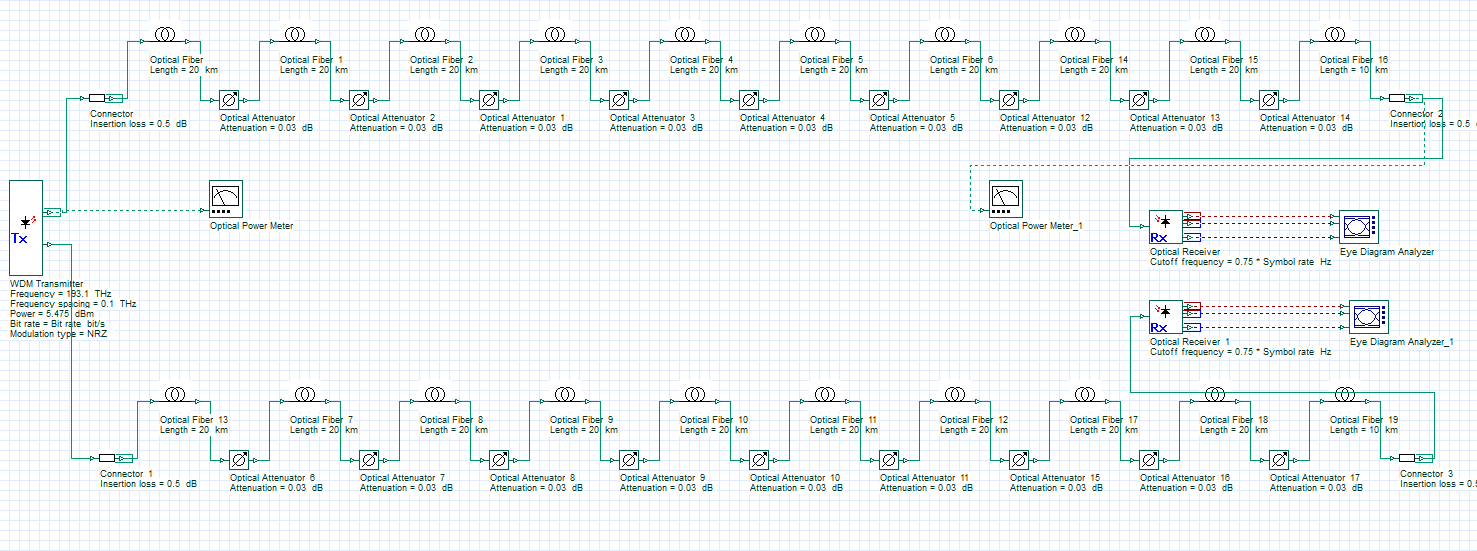
\includegraphics[width=0.9\linewidth]{img/Figure_6_1}
			\caption{Esquema global en OptiSystem para la situacion sin amplificador una linea de 190Km}
			\label{fig:9}
		\end{figure}
		\begin{figure}
			\centering
			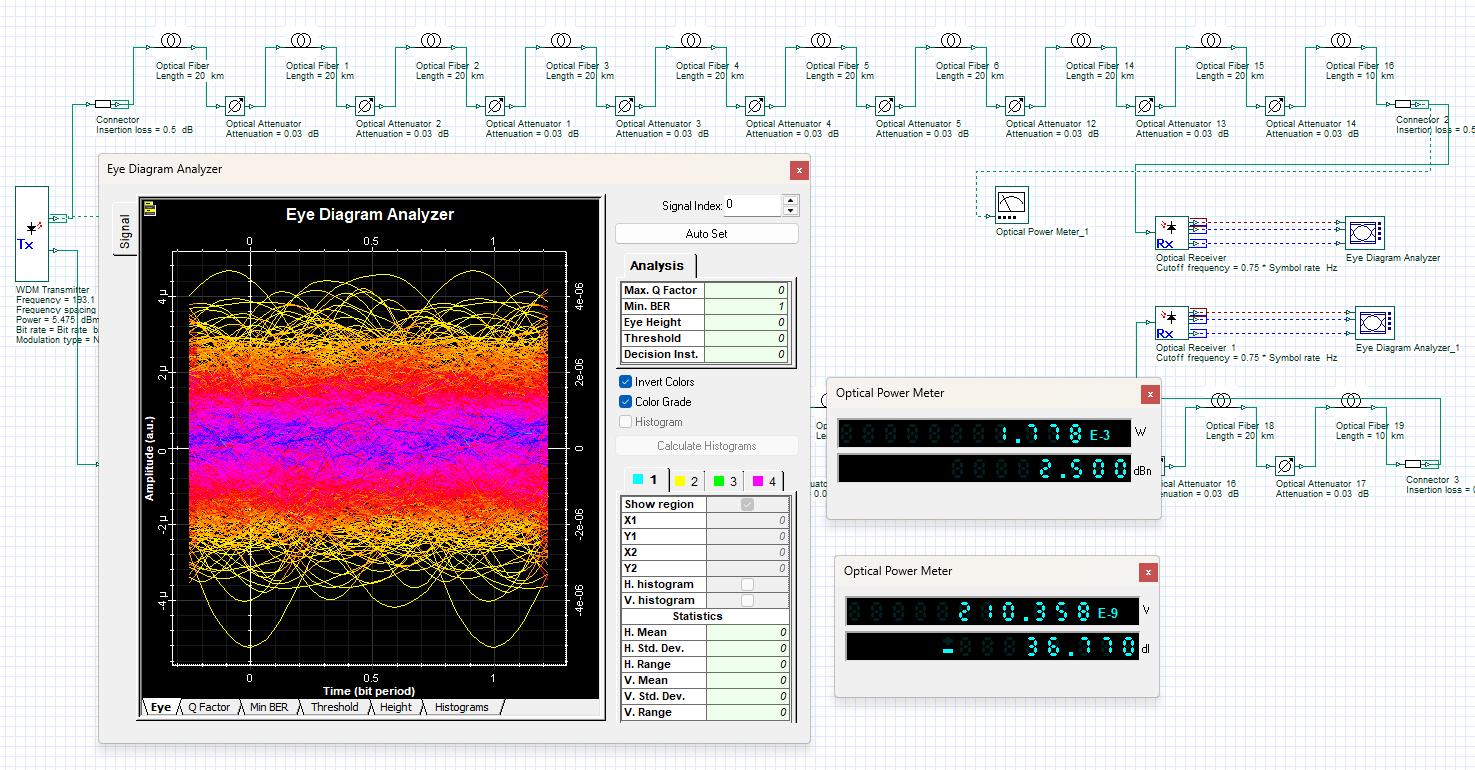
\includegraphics[width=0.9\linewidth]{img/Figure_6_2}
			\caption{Visualizacion de la potencia de entrada, salida y el diagrama de Ojos para la situacion sin amplificador una linea de 190Km}
			\label{fig:10}
		\end{figure}
		Luego se considera el sistema con amplificador para el caso de 190 km con amplificador, con lo que se obtiene:
		\begin{figure}
			\centering
			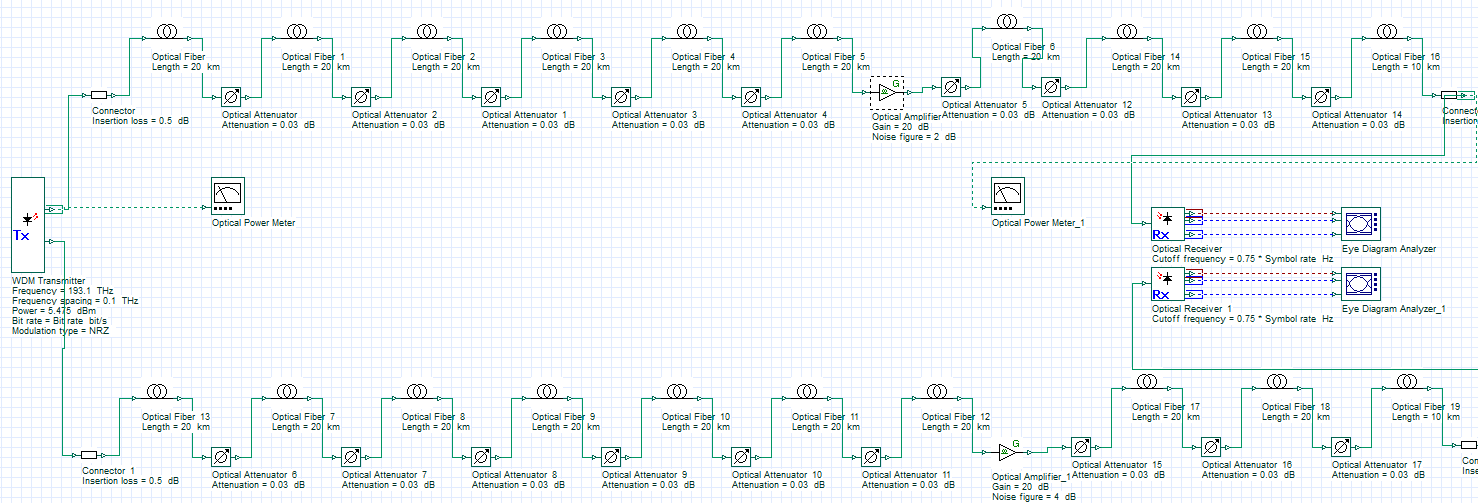
\includegraphics[width=0.9\linewidth]{img/Figure_6_3}
			\caption{Esquema global en OptiSystem para la situacion con amplificador una linea de 190Km}
			\label{fig:11}
		\end{figure}
		\begin{figure}
			\centering
			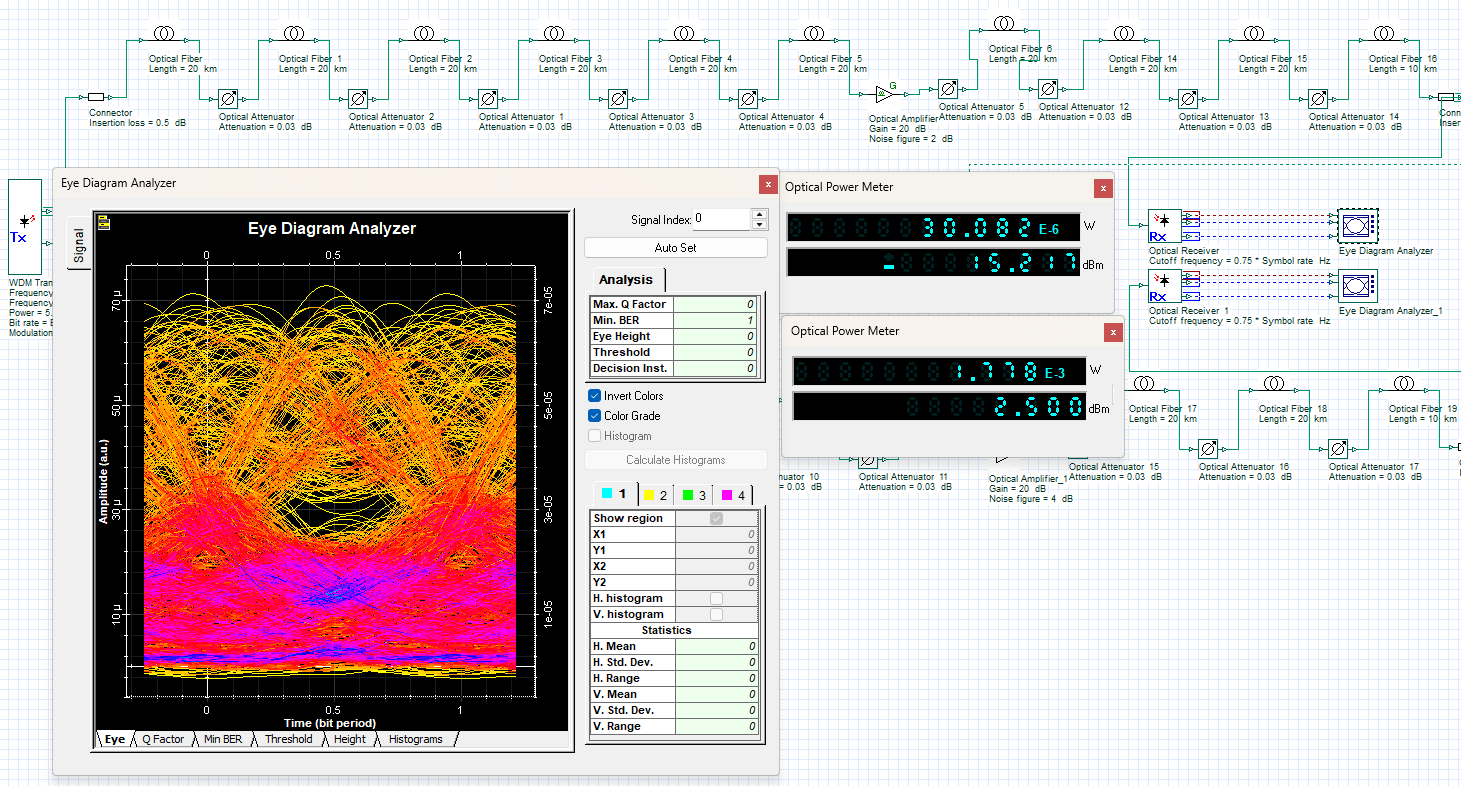
\includegraphics[width=0.9\linewidth]{img/Figure_6_4}
			\caption{Visualizacion de la potencia de entrada, salida y el diagrama de Ojos para la situacion con amplificador una linea de 190Km}
			\label{fig:12}
		\end{figure}
		Con lo que se puede concluit que el efecto del amplificador es significativo en la calidad de la señal, mejorando la claridad y la integridad de la transmisión en un enlace de 190 km que corresponde con lo esperado de manera teorica realizada previamente.
		\item Capturas de pantalla de Diagrama de Ojo con amplificador y sin amplificador. Compare las formas y Analice el BER, luego concluya.
		Es posible el realizar una comparacion entre ambos casos para el diagrama de ojo, para esto se tiene que:
		\begin{figure}
			\centering
			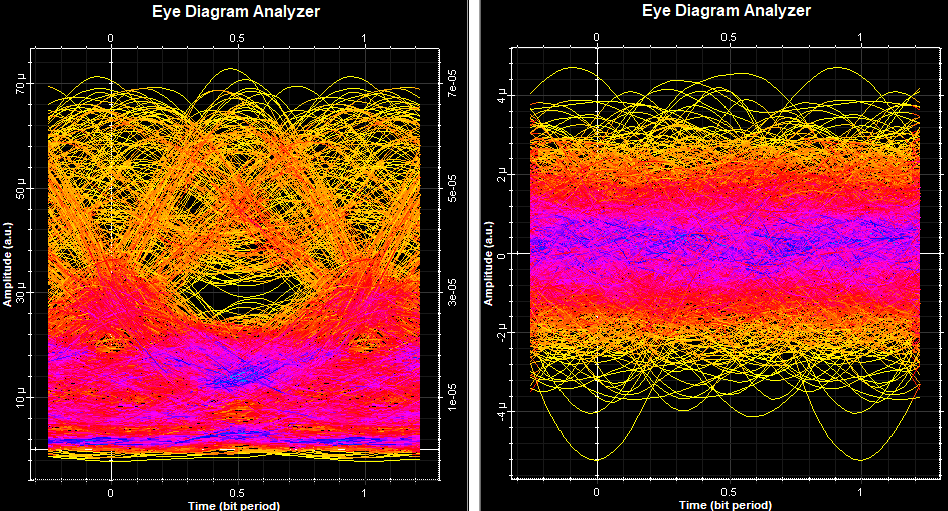
\includegraphics[width=0.9\linewidth]{img/Figure_6_5}
			\caption{Comparacion de los diagramas de ojos para los casos con y sin amplificador}
			\label{fig:13}
		\end{figure}
	\end{itemize}
	El análisis comparativo entre el sistema con y sin amplificador EDFA demuestra la importancia de la amplificación para mantener la integridad de la señal en largas distancias. Sin amplificación, el diagrama de ojo presenta una apertura muy limitada, lo que indica una señal con alto nivel de ruido y distorsión. Esta falta de claridad entre los niveles lógicos genera una alta tasa de error de bits (BER), lo cual hace que el enlace sea ineficiente y poco confiable para cubrir una distancia de 190 km. En contraste, con el amplificador EDFA, el diagrama de ojo muestra una apertura significativamente mayor, reflejando una señal mucho más clara y estable.Por lo tanto, el uso del amplificador resulta esencial para alcanzar el rendimiento óptico necesario en un enlace DWDM de larga distancia.
\end{enumerate}